\chapter{ ROCKET: RandOm Convolutional KErnel Transform}
In questo capitolo andremo ad analizzare gli algoritmi di nostro interesse, ossia ROCKET e ROCKAD.
Questi algoritmi lavorano con le timeseries, le quali sono una sequenza di dati registrati ad intervalli di tempo consecutivi. Ogni punto della serie è associato ad un timestamp, il quale indica il momento in cui è stato registrato.

ROCKET, ancora non utilizzato per il rilevamento delle anomalie, è stato selezionato come nuovo algoritmo, per la sua grande capacità di estrarre caratteristiche importanti dalle serie temporali e per l'efficienza di utilizzo.
Tutto questo è reso possibile grazie anche ai kernel casuali che non necessitano di grande capacità di calcolo, rispetto ad altri algoritmi più complessi.

Ciò che garantisce la robustezza di ROCKET sono i kernel casuali e le tecniche di pooling che vi si possono applicare, portando così a poter eliminare la necessità di ottimizzare gli iperparametri.
ROCKET viene descritto come efficiente e scalabile anche su grandi dataset, oltre ad un fattore di adattabilità ai dataset con caratteristiche variabili, molto elevato.

L'obbiettivo principale è utilizzare ROCKET per il rilevamento delle anomalie direttamente a bordo dei satelliti, riducendo la necessità di scambiare informazioni con la stazione centrale e minimizzando i falsi positivi.

Dopo l'uscita di ROCKET e valutata la sua efficacia è stato introdotto ROCKAD (Random Convolutional Kernel Transform Anomaly Detector), questo è un estensione di ROCKET progettata appositamente per il rilevamento delle anomalie.

Secondo gli sviluppatori, ROCKAD permette di ottenere un rilevamento di anomalie più preciso e mirato, sfruttando le caratteristiche estratte da ROCKET.
ROCKAD trova maggiore spazio in contesti in cui l'etichettatura dei dati è limitata o assente (come vedremo per NASA), consentendo una classificazione basata su punteggi di anomalia.

\section{ROCKET}
ROCKET è un algoritmo convoluzionale, questo è anche detto rete neurale convoluzionale (CNN). Questi algoritmi lavorano su dati con una struttura a griglia come immagini e serie temporali e sono progettati per riconoscere pattern all'interno dei dati tramite operazioni di convoluzione.
Vengono utilizzati i kernel\footnote{Matrice di pesi usata per eseguire operazioni di filtraggio per estrarre caratteristiche specifiche, opera tramite moltiplicazioni e addizioni}, che operando sui dati in input estraggono caratteristiche locali dei dati (features); in questa fase possono essere applicate tecniche di centratura, ovvero aggiungere dei bordi attorno all'input, così da mantenere le dimensioni dopo aver applicato il kernel, questo si chiama padding.

Ci sono tecniche applicabili a ROCKET come il pooling, che ha lo scopo di ridurre la dimensione e quindi di rendere l'algoritmo meno sensibile alle traslazioni. In merito a questo vediamo le due tecniche più utilizzate:
\begin{itemize}
    \item Max Pooling: prende solo il valore massimo in una finestra specifica riducendo la dimensione dell'input;
    \item Average Pooling: riduce la dimensione prendendo la media dei valori in una finestra;
    \item Proportion of Positive Value (PPV): calcola la percentuale di valori positivi nell'output della convoluzione, individuando quanto spesso il kernel produce valori maggiori di zero.
\end{itemize}

In conclusione abbiamo il passaggio per gli strati: i dati vengono appiattiti (flattening) fatti passare attraverso uno o più strati completamente connessi per la classificazione o la regressione, in modo da ottenere il risultato desiderato.

ROCKET in particolare utilizza i kernel convoluzionali casuali, generandone un gran numero con iperparametri scelti casualmente, come lunghezza del kernel, Dilatation Rate, Bias e pesi dei kernel.
Questi kernel filtrano i dati delle serie temporali producendo una serie di features. Utilizzando tecniche di pooling viste in precedenza, otteniamo statistiche riassuntive da queste features.
La procedura viene ripetuta per tutti i kernel, portando ad un enorme quantità di caratteristiche e quindi una maggiore possibilità di estrarre tutti i pattern comuni.

Le caratteristiche estratte vengono poi date in input ad algoritmi di classificazione, tipicamente una regressione logistica data la sua scalabilità e velocità su grandi dataset.
L'algoritmo viene addestrato su questi elaborati per effettuare la classificazione delle serie temporali.

Per rendere più chiara la logica di funzionamento prendiamo in considerazione la Figura \ref{fig:rocket_paper}, presa dal paper di ROCKAD$^{\text{\cite{rockad_paper}}}$.
Come possiamo osservare, in ingresso ROCKET prende la timeseries di una specifica features $T$, e tramite moltiplicazioni tra matrici, chiamate filtri (kernel), otteniamo un array di caratteristiche di $2K$ features ($K$ features per ogni tecnica di pooling utilizzata).
Questo processo viene ripetuto per ogni features del dataset, portando ad avere un numero di caratteristiche pari a 10.000 volte il numero di features iniziali (nel caso di kernel di default).

\begin{figure}[!ht]
    \centering
    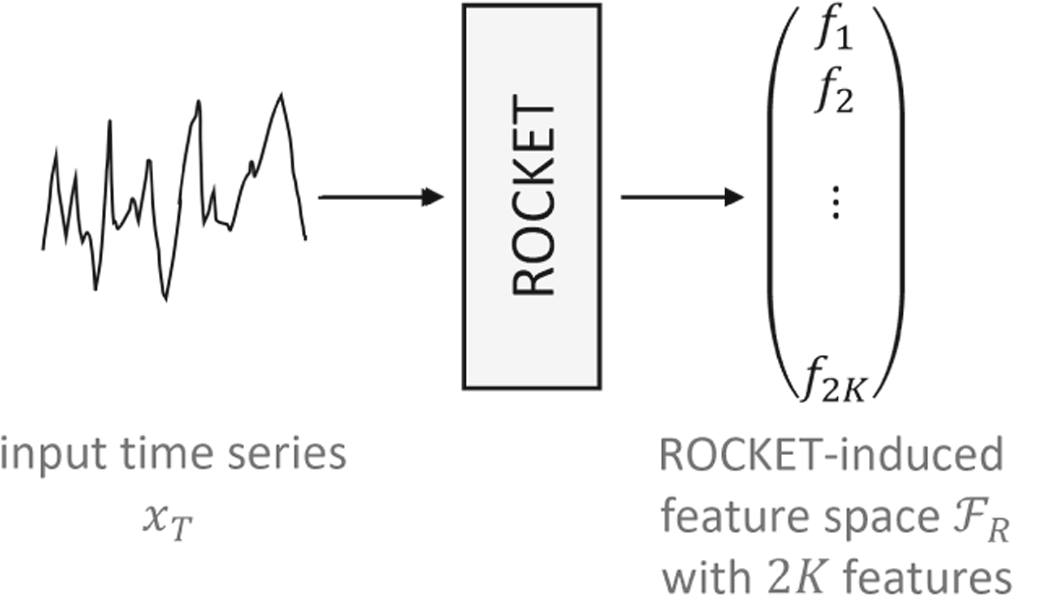
\includegraphics[width=0.5\linewidth]{images//Capitolo4/ROCKET_Paper.png}
    \caption{Funzionamento ROCKET}
    \label{fig:rocket_paper}
\end{figure}

ROCKET quindi scorre la timeseries con delle finestre di dimensione uguale tra loro, come possiamo vedere dalla Figura \ref{fig:rocket_finestre}. Le caratteristiche estratte da ciascuna finestra vengono successivamente utilizzate da un classificatore, che elabora tali informazioni per fornire una predizione sull'intera serie temporale relativa alla feature originale.

\begin{figure}[!ht]
    \centering
    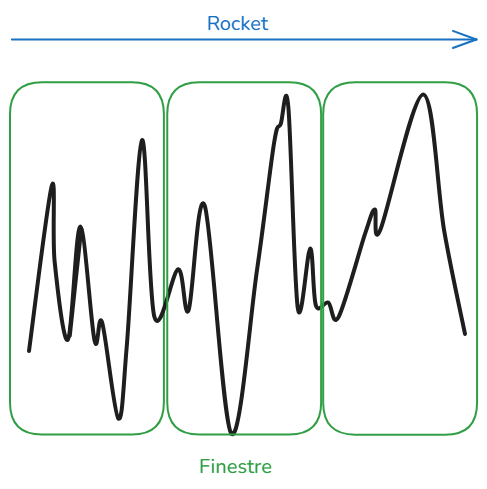
\includegraphics[width=0.5\linewidth]{images//Capitolo4/ROCKET_finestre.png}
    \caption{Finestre ROCKET su timeseries}
    \label{fig:rocket_finestre}
\end{figure}
\pagebreak
\subsection{Aspetti Tecnici}
Per implementare ROCKET abbiamo usato la libreria utilizzata anche dal paper di ROCKAD tramite:
\begin{lstlisting}[language=Python]
from sktime.transformations.panel.rocket import Rocket
\end{lstlisting}
I parametri più importanti sono:
\begin{itemize}
    \item Numero di kernel (num\textunderscore kernels): rappresenta il numero di kernel casuali da generare, il valore predefinito è 10.000, un numero maggiore di kernel tende a migliorare l'accuratezza della classificazione, di conseguenza aumenta la complessità e quindi il tempo di calcolo;
    \item Lunghezza del kernel (input\textunderscore length): rappresenta la lunghezza del singolo kernel, questa è casuale e determina quanto, della serie temporale, viene considerato durante la convoluzione;
    \item Dilatazione: è un parametro che controlla la distanza tra i punti analizzati nel kernel; ROCKET usa varie dilatazioni per catturare caratteristiche di diverse scale temporali;
    \item Padding: determina come vengono gestiti i bordi delle serie temporali durante la fase di convoluzione.
\end{itemize} 

I vantaggi di ROCKET sono:
\begin{itemize}
    \item Efficienza computazionale elevata: è progettato per essere estremamente veloce e scalabile in modo che possa gestire grandi dataset in tempi ristretti;
    \item Robustezza: dato che si basa su kernel casuali, consente di generalizzare bene su nuovi problemi, senza la necessità di perfezionare gli iperparametri;
    \item Semplicità: ROCKET permette di usare un solo iperparametro, ossia il numero di kernel, riducendo così la complessità associata al perfezionamento rispetto ad altri metodi di classificazione delle serie temporali.
\end{itemize}
\subsection{Metodologia Applicata}
Nel paper di ROCKET$^{\text{\cite{paper_rocket}}}$, esso viene applicato, in particolare per la classificazione delle serie temporali, portando a sostegno molteplici valutazioni su dataset di BakeOff. Partendo da queste analisi e valutazioni del modello sulle serie temporali vogliamo riprodurre tali dati, molto promettenti, per la prima volta utilizzando ROCKET con lo scopo di classificazione delle anomalie sulle serie temporali.

% ================ Da vedere come e se scrivere in base a mail e funzionamento
Un aspetto da considerare è la formattazione dei dati che utilizziamo, infatti estraendo i dati dal dataset grezzo di OPS\textunderscore SAT e elaborandoli, come vedremo meglio nella parte relativa a ROCKAD, in modo che siano compatibili con ROCKET.

\subsection{Test Effettuati}
Come primo aspetto abbiamo eseguito in locale gli esperimenti del paper di ROCKET per avere una validazione empirica dell'algoritmo, ottenendo risultati compatibili con quelli della tabella del paper$^{\text{\cite{paper_rocket}}}$; successivamente abbiamo testato la nostra implementazione sui medesimi dataset ottenendo i risultati della Tabella \ref{tab:Rocket_paper}.
\begin{table}[h!]
    \centering
    \begin{adjustbox}{max width=\textwidth}
        \begin{tabular}{|c|c|}
            \hline
            \textbf{Dataset} & \textbf{Accuracy}\\
            \hline
             Coffee &1.0 \\
             \hline
             Computers& 0.64\\
             \hline
             Adiac& 0.634\\
             \hline
             ArrowHead& 0.788\\
             \hline
             BeetleFly& 0.8\\
             \hline
             CinCECGTorso& 0.7898\\
             \hline
             CBF& 0.971\\
             \hline
             ChlorineConcentration& 0.590\\
             \hline
             GunPoint& 0.9866\\
             \hline
             Ham& 0.771\\
             \hline
             HandOutlines& 0.935\\
             \hline
             InlineSkate& 0.367\\
             \hline
             Lightning2& 0.623\\
             \hline
             Mallat& 0.928\\
             \hline
             MiddlePhalanxTW& 0.558\\
             \hline
        \end{tabular}
    \end{adjustbox}
    \caption{Esecuzione di ROCKET su dataset "BakeOff"}
    \label{tab:Rocket_paper}
\end{table}
\pagebreak

Nei risultati che osserveremo in seguito nella Tabella \ref{tab:RocketOPS_SAT}, sono state effettuate molte prove con varie modalità.
La prima è unsupervised, ovvero utilizziamo ROCKET per estrarre una grande quantità di caratteristiche e, tramite una threshold, fare una classificazione binaria senza aver effettuato un training con le etichette dei risultati.
Una threshold è una soglia, che indica il valore di riferimento per decidere quando una predizione deve essere classificata come positiva o negativa, in questo caso segnala quando un valore deve essere considerato o no anomalo.
La seconda modalità che abbiamo osservato è supervised, effettuando quindi il training sulle features trovate da ROCKET passando però le etichette delle classificazioni.
Per questo abbiamo utilizzato vari algoritmi supervised per analizzare le varie performance e trovare il migliore.
Abbiamo anche osservato una modalità ibrida, ossia al posto dell'utilizzo di una threshold o un algoritmo supervised abbiamo puntato su uno unsupervised (KNN) facendo il training sulle features e restituendo delle prediction e delle classificazioni; il KNN, solitamente usato in modo supervised, nel nostro caso è stato utilizzato per calcolare la distanza dai $k$ vicini più prossimi e assegnando un punteggio di anomalia basato su queste distanze.

\texttt{RidgeClassifierCV}: è il modello di classificazione usato come standard nel paper di ROCKET; nel nostro caso utilizzandolo con il dataset OPS\textunderscore SAT abbiamo riscontrato metriche migliori in tutti i test.
\begin{table}[h!]
    \centering % Correttamente posizionato
    \begin{adjustbox}{max width=\textwidth}
        \begin{tabular}{|c|c|c|c|c|c|c|c|c|c|}
        \hline
        \textbf{Modalità} & \textbf{Accuracy} &\textbf{Precision}  & \textbf{Recall} & \textbf{F1} & \textbf{MCC} & \textbf{AUC-PR} & \textbf{AUC-ROC} & \textbf{NScore}&\textbf{Tempo}\\
        \hline
        \multicolumn{10}{|c|}{\textbf{Unsupervised}} \\
        \hline
        \textbf{Threshold} & 0.546 & \textbf{1.0} & 0.048 &0.092  & 0.161 & 0.46 & 0.468 & 0.419 &7s \\
        \hline
        \multicolumn{10}{|c|}{\textbf{Supervised}} \\
        \hline
         \textbf{RidgeCV} &\textbf{ 0.777} & 0.704 & \textbf{0.919} &\textbf{0.797}  & \textbf{0.584} & 0.787& 0.829 &0.726&6.6s \\
        \hline
        \textbf{LogisticReg} & \textbf{0.777} & 0.704 & \textbf{0.919} &\textbf{0.797}  &\textbf{ 0.584} & 0.773& 0.837 &\textbf{0.774} &53.3s\\
        \hline
        \textbf{RidgeReg} & 0.538 & \textbf{1.0} & 0.032 &0.062  & 0.131 & \textbf{0.779}& \textbf{0.844} &0.758 &5.8s \\
        \hline
        \multicolumn{10}{|c|}{\textbf{Ibrid Unsupervised}} \\
        \hline
        \textbf{KNN} & 0.531 & 0.6 & 0.048 &0.09  & 0.049 & 0.407& 0.294 &0.29 & 9.4s \\
        \hline
        \end{tabular}
    \end{adjustbox}
    \caption{Algoritmi eseguiti su dataset OPS\textunderscore SAT}
    \label{tab:RocketOPS_SAT}
\end{table}


\pagebreak

\subsection{Implementazione}

Riportiamo qui il codice dell'implementazione degli algoritmi più importanti.
Il primo rappresenta ROCKET con la threshold come decision function:
\lstinputlisting{listings/Capitolo4/RocketThreshold.py}
\pagebreak
La seconda implementazione è quella relativa a ROCKET con RidgeClassifierCV:
\lstinputlisting{listings/Capitolo4/RocketRidgeClassifierCV.py}

% ===============================================================================
% ================================= ROCKAD ======================================
% ===============================================================================
\pagebreak
\section{ROCKAD}
ROCKAD (Random Convolutional Kernel Transform Anomaly Detector) è un algoritmo basato su ROCKET per la classificazione di anomalie su serie temporali.
\subsection{Funzionamento}
La logica dietro a questo algoritmo è spezzata in due parti che sfruttano due modelli: nella prima è utilizzato ROCKET come estrattore di caratteristiche; nella seconda viene addestrato un singolo KNN o un insieme combinato di più KNN (detto ensemble di KNN).

In modo più dettagliato ROCKAD è diviso in tre passaggi fondamentali:
\begin{enumerate}
    \item Estrazione di caratteristiche: tramite ROCKET ricaviamo le caratteristiche delle timeseries;
    \item Trasformazione: le caratteristiche estratte vengono poi trasformate utilizzando un power trasformer;
    \item Rilevamento anomalie: per concludere viene addestrato un insieme di KNN sulle caratteristiche estratte per calcolare dei punteggi di anomalia (score) per le serie temporali che serviranno successivamente per ottenere le predizioni (KNN in questo caso è unsupervised).
\end{enumerate}

I parametri principali di ROCKAD sono tre: il numero di kernel convoluzionali (il valore predefinito è 10.000), il numero di estimatori di tipo KNN (il valore predefinito è 10) e il numero di vicini che vengono utilizzati per calcolare il punteggio di anomalia (il valore predefinito è 5).

Oltre alla classe ROCKAD è necessario importare anche la classe NearestNeighborOCC, che implementa un classificatore di anomalie basato sul nodo prossimo più vicino.
Questo è un metodo aggiuntivo per il rilevamento delle anomalie, il quale ha un funzionamento diverso dal KNN classico, dato che, invece di utilizzare la distanza media dai $k$ vicini più prossimi, NearestNeighborOCC calcola un punteggio di anomalia basato sul rapporto tra due distanze:
\begin{enumerate}
    \item la distanza tra lo score della timeseries $t$ analizzata e il suo vicino prossimo $v$;
    \item la distanza tra il vicino $v$ e il suo vicino più prossimo $r$.
\end{enumerate}
Se il risultato di questo rapporto è inferiore o uguale ad $1$, la timeseries viene classificata come normale, altrimenti come anomala.

In conclusione NearestNeighborOCC aggiunge un ulteriore passaggio di analisi per la classificazione, il quale permette di aumentare la robustezza e l'accuratezza nel rilevamento delle anomalie, classificando lo score estratto come anomalie a o meno.
\subsection{Validazione}
Nel paper relativo a ROCKAD$^{\text{\cite{rockad_paper}}}$ sono paragonati i risultati ottenuti con il suo utilizzo e il confronto con gli altri algoritmi. Nel nostro caso, come per  ROCKET, validiamo l'algoritmo con i dati presenti nella Tabella \ref{tab:rockad_paper_table}, per poi concentrarci sulla sua applicazione sui nostri dataset di riferimento.

\begin{table}[h!]
    \centering
    \begin{tabular}{|c|c|}
        \hline
        \textbf{Dataset} & \textbf{AUC-ROC}\\
        \hline
         GunPoint &0.9792 \\
         \hline
         CBF& 1.0\\
         \hline
         BME& 1.0\\
         \hline
         ArrowHead& 0.852\\
         \hline
         Computers& 0.808\\
         \hline
         ChlorineConcentration& 0.655\\
         \hline
         Ham& 0.486\\
         \hline
         InlineSkate& 0.637\\
         \hline
         Lightning2& 0.623\\
         \hline
         Mallat& 1.0\\
         \hline
         CricketX& 0.760\\
         \hline
         Crop& 0.999\\
         \hline
         CricketX& 0.760\\
         \hline
         Fish& 0.933\\
         \hline
    \end{tabular}
    \caption{Esecuzione locale ROCKAD}\label{tab:rockad_paper_table}
\end{table}
\pagebreak

\subsection{Preprocessing del Dataset OPS\textunderscore SAT}
Come prima cosa, per poter ottenere i risultati sul dataset OPS\textunderscore SAT, bisogna manipolare i dati per renderli compatibili con ROCKAD.
I dati accettati dai metodi \texttt{fit} e \texttt{predict\textunderscore proba} sono di tipo \texttt{numpy.array}.

Siamo partiti estraendo i dati grezzi provenienti da OPS-SAT nel file \\ \texttt{segments.csv}, eseguendo un preprocessing per strutturarli in modo tale che abbiano una forma del tipo  \texttt{(numero esempi, numero di features, lunghezza sequenza)}. Nel nostro caso abbiamo fissato la lunghezza della sequenza a $250$ e il numero di features ad 1 per avere la compatibilità con ROCKAD, quindi eseguendo la funzione \texttt{.shape} dovrebbe risultare $(347, 1, 250)$ dove 347 è il numero di esempi.

I dati processati vengono poi passati a ROCKAD, suddivisi in due parti: una per il fitting del modello e l'altra per calcolare gli \textit{score\textunderscore train} e gli \textit{score\textunderscore test}. Questi punteggi vengono successivamente utilizzati rispettivamente per il training e la predizione dell'algoritmo NearestNeighborOCC, al fine di calcolare le predizioni e confrontarle con i \textit{ground\textunderscore truth}.

% Mettere l'errore e la risoluzione del problema???

Il codice del preprocessing è diviso in due: 

\begin{itemize}
    \item la parte riguardante i dati di training

\end{itemize}
\lstinputlisting{listings/Capitolo4/PreprocessingTrain.py}
\begin{itemize}
    \item la parte corrispondente ai dati di test
\end{itemize}
\lstinputlisting{listings/Capitolo4/PreprocessingTest.py}



% Descrizione delle prove effettuate con ROCKAD su OPS_SAT
\subsection{Test Effettuati su OPS\textunderscore SAT}
Una volta effettuata la parte di preprocessing possiamo utilizzare i dati appena modificati per allenare ROCKAD ed effettuare la classificazione con NearestNeighborOCC.
Come prima cosa inizializziamo il modello importando le classi ROCKAD e NearestNeighborOCC estratte dall'implementazione fornita con il paper ROCKAD$^{\text{\cite{rockad_paper}}}$.
Una volta effettuato possiamo passare a ROCKAD i dati di training per il fitting e calcoliamo con \texttt{predict\textunderscore proba} gli score relativi al training set.
Gli score di training sono poi passati a NearestNeighborOCC come dati di input per il suo allenamento, successivamente sono stati processati gli score di test, sui quali eseguiamo la \texttt{predict} con la quale otteniamo i valori risultanti che ci indicano quali sotto sequenze della timeseries sono anomale e quali invece no.

Effettuando vari test abbiamo osservato che il miglior numero per \texttt{n-neighbors} è quello di default, ossia uguale a 5.

Per il numero di estimatori sono stati effettuati molteplici test riportando i risultati nella Tabella \ref{tab:ROCKAD_OPS-SAT}, dove il primo valore della tupla della colonna "Modalità" indica il numero di estimatori ed il secondo quello dei kernel.

\begin{table}[h!]
    \centering
    \begin{adjustbox}{max width=\textwidth}
    \begin{tabular}{|c|c|c|c|c|c|c|c|c|c|}
    \hline
         \textbf{Modalità} & \textbf{Accuracy} &\textbf{Precision}  & \textbf{Recall} & \textbf{F1} & \textbf{MCC} & \textbf{AUC-PR} & \textbf{AUC-ROC} & \textbf{N-Scores}&\textbf{Tempo}\\
        \hline
        (10, 1000) &0.492& 0.476& 0.645& 0.548&-0.002& 0.755 &0.702 & 0.677 & 1m 49s \\
         \hline
         (10, 5000) &0.538& 0.514& 0.613& 0.559&0.084& 0.76 &0.705 & 0.677&1m 52.7s\\
         \hline
        (10,10.000)&\textbf{0.546} &\textbf{0.515} &\textbf{0.823} &\textbf{0.634} & \textbf{0.137}& 0.757& 0.704&0.677& 2m 12.5s\\
         \hline
         (20,10.000)&0.454 &0.447 &0.613 &0.517 &-0.082 &0.758 &0.705& 0.677&2m 37.4s\\
         \hline
         (30,10.000)&0.508 &0.489 &0.71 &0.579 &0.036 &\textbf{0.762} &\textbf{0.709}& 0.677& 3m 17.1s\\
         \hline
         (35,10.000)&0.515 &0.494 &0.71 &0.583 & 0.052 &\textbf{0.762} &0.708& 0.677&3m 31s\\
         \hline
         (40,10.000)&0.531 &0.506 &0.71 &0.591 &0.082 &\textbf{0.762} &0.707& 0.677&3m 44.2s\\
         \hline
         (10,20.000)&0.538 &0.513 &0.645 &0.571 &0.088 &0.758 &0.705& 0.677&2m 52.3s\\
         \hline
    \end{tabular}
    \end{adjustbox}
    \caption{Test con numero di estimatori e kernel variabile}
    \label{tab:ROCKAD_OPS-SAT}
\end{table}

% da aggiungere alemeno una prova con 20.000 kernel ed una con 1000 ossia quello di default
\pagebreak

\section{Problematiche}
Nonostante le caratteristiche ed i vantaggi di ROCKET e ROCKAD, rimangono sempre alcune problematiche che possono essere riscontrate.
Nel caso di ROCKET abbiamo la ridondanza di caratteristiche che porta ad un aumento di probabilità di avere un overfitting su dataset di piccole dimensioni.
Per ROCKAD, dato il modello aggiuntivo KNN, richiede più potenza di calcolo per gestirlo, ma anche la trasformazione delle caratteristiche che avviene internamente richiede più risorse.
Per finire, come ulteriore problematica, entrambi gli algoritmi rendono complessa l'analisi dettagliata dei risultati data la limitata accessibilità delle caratteristiche estratte.

\pagebreak

% aggiungere implementazione ROCKAD

\section{Test NASA}
Per verificare in maniera più completa le performance di ROCKET e ROCKAD, utilizziamo anche il dataset NASA.
L'integrazione di questi algoritmi con il dataset, avviene in parte tramite l'uso di codice nel repository GitHub di SpaceAI$^{\text{\cite{SpaceAI}}}$: come prima cosa vengono scaricati i dati, se non già presenti, da una risorsa remota
tramite due modi diversi, chiamati "prediction" e "anomaly", che rispettivamente si usano per estrarre i dati delle serie temporali e per prendere i valori anomali nella timeseries.
Successivamente dobbiamo spezzare la timeseries in sotto sequenze, così da poterla utilizzare con i kernel casuali di ROCKET per generare le features.

Effettuiamo gli stessi passaggi per l'estrazione e l'elaborazione dei dati di test e per i valori delle predizioni attese, ossia i \textit{ground truth}; questi devono essere creati, dato che l'estrazione tramite la funzione è sotto forma di insieme, dove si evidenziano solo gli estremi tra i quali la timeseries è anomala.
Questa lista viene spezzata in sottoliste di 250 elementi, che possono essere 0 o 1; per ottenere un valore per ogni timeseries è necessario applicare un metodo per scegliere se una sottolista è anomala o no, in base al numero di elementi uguali ad 1. 
Nel nostro caso abbiamo utilizzato una soglia fissata a 25, cioè almeno 25 elementi uguali ad 1 in una sottolista.

Qui sotto è stato riportata l'implementazione della parte di codice relativa all'estrazione dei dati e la relativa formattazione per rendere compatibili i dati.

\lstinputlisting{listings/Capitolo5/NASA_preprocessing.py}

Arrivati a questo punto abbiamo tutti i dati che ci servono per utilizzare ROCKET e ROCKAD, che però dovranno essere applicati ciclicamente a tutti i canali del dataset; per ognuno di questi vengono valutate le metriche che serviranno per calcolare le metriche effettive di tutto il dataset, facendo una media tra tutti i risultati dei canali.

Poniamo particolare attenzione all'utilizzo dell'OFFSET introdotto per utilizzare al meglio ROCKAD e ROCKET sul dataset NASA, dato che le timeseries di alcuni canali sono molto corte e non permettono di utilizzare il KNN come classificatore mantenendo il numero di nodi vicini mantenendo il valore di default.

Tramite l'uso dell'OFFSET in combinazione con la variabile STEP, permette di prendere finestre della stessa dimensione spostandosi solo del valore indicato nell'OFFSET, portando così ad avere overlapping, ossia due finestre che condividono alcuni elementi.
Tutto ciò porta ad avere un maggior numero di finestre con lo stesso numero di esempi di partenza (Figura \ref{fig:OFFSET_STEP}).

\begin{figure}[!ht]
    \centering
    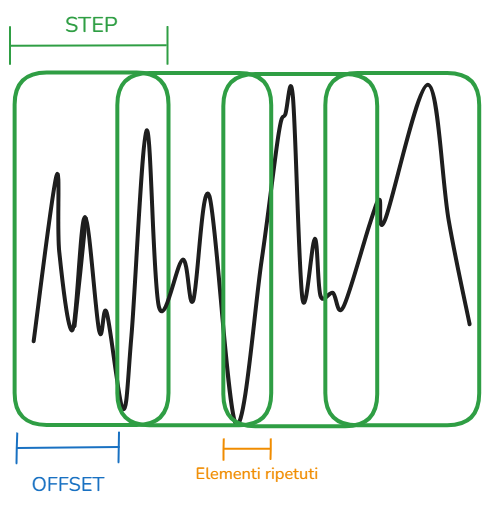
\includegraphics[width=0.5\linewidth]{images//Capitolo4/OFFSET_STEP.png}
    \caption{Finestre ROCKET su timeseries con OFFSET}
    \label{fig:OFFSET_STEP}
\end{figure}

\subsection{Metriche Rilevate}
In questo paragrafo riportiamo le metriche riscontrate dell'esecuzione di ROCKET e ROCKAD con diversi valori di: numero di kernel, valore di OFFSET e numero di n\textunderscore neighbors.

Le metriche, data la conformazione del dataset, sono divise per canale, questo porta ad una scelta che bisogna effettuare, ossia come calcolare le metriche.
Per uniformare i valori delle metriche, in particolare dell'F1, scegliamo di conservare in un file \textit{.json} tutti i valori necessari (TP, TN, FP, FN) per calcolare le metriche dopo l'analisi di tutti i channel, ritardando così il calcolo.
Riportiamo queste metriche nella Tabella \ref{tab:NASA_Posticipato}.
Un'altra possibile soluzione prevede di calcolare subito le metriche di ogni canale e poi fare la media alla fine di tutte le metriche, questo calcolo è meno accurato e tende a produrre metriche minori, riportiamo comunque i risultati ottenuti nella Tabella \ref{tab:NASA_Media}.

\begin{table}[!ht]
    \centering % Correttamente posizionato
    \begin{adjustbox}{max width=\textwidth}
        \begin{tabular}{|c|c|c|c|c|c|c|c|}
        \hline
        \textbf{Accuracy} &\textbf{Precision}  & \textbf{Recall} & \textbf{F1} & \textbf{MCC} & \textbf{AUC-PR} & \textbf{AUC-ROC} & \textbf{NScore}\\
        \hline
        \multicolumn{8}{|c|}{\textbf{ROCKET}} \\
        \hline
        \multicolumn{8}{|c|}{kernel=10.000, n\textunderscore neighbors=1 e OFFSET=50} \\
        \hline
         \textbf{0.735} & \textbf{0.299} & 0.471 &0.366  & \textbf{0.232 }& 0.286& 0.652 & 0.378 \\
        \hline
        \multicolumn{8}{|c|}{kernel=10.000, n\textunderscore neighbors=2 e OFFSET=30} \\
        \hline
         0.719 & 0.284 & \textbf{0.482} &0.357  & 0.219 & 0.28& 0.647 & 0.371 \\
        \hline
        \multicolumn{8}{|c|}{kernel=1000, n\textunderscore neighbors=1 e OFFSET=50} \\
        \hline
         0.731 & 0.296 & 0.478 &\textbf{0.367}  & 0.231 & \textbf{0.288}& \textbf{0.654} & \textbf{0.384} \\
        \hline
        \multicolumn{8}{|c|}{kernel=1000, n\textunderscore neighbors=2 e OFFSET=30} \\
        % da cambiare
        \hline
         0.721 & 0.284 & 0.473 &0.355  & 0.217 & 0.281& 0.647 & 0.37 \\
        \hline
        \multicolumn{8}{|c|}{kernel=1000, n\textunderscore neighbors=5 e OFFSET=10} \\
        % da cambiare
        \hline
         0.730 & 0.295 & 0.477 &0.365  & 0.230 & 0.278& 0.648 & 0.382 \\
         \hline
        \multicolumn{8}{|c|}{\textbf{ROCKAD}} \\
        \hline
        \multicolumn{8}{|c|}{kernel=10.000, n\textunderscore neighbors=1 e OFFSET=50} \\
        \hline
        \textbf{0.593} & 0.106 & 0.19 &0.136  & -0.129 &0.287 &\textbf{0.651}  &0.378 \\
        \hline
        \multicolumn{8}{|c|}{kernel=10.000, n\textunderscore neighbors=2 e OFFSET=30} \\
        \hline
        0.628 & \textbf{0.131} & 0.207 &0.16  & \textbf{-0.076} &\textbf{0.29} &0.646  &0.379 \\
        \hline
        \multicolumn{8}{|c|}{kernel=1000, n\textunderscore neighbors=2 e OFFSET=50} \\
        \hline
        0.6 & 0.106 & 0.193 &0.137  & -0.131 &0.286 &\textbf{0.651}  &0.378 \\
        \hline
        \multicolumn{8}{|c|}{ROCKAD con 1000 kernel, n\textunderscore neighbors=2 e OFFSET=30} \\
        \hline
        0.614 & 0.129 & \textbf{0.218} &\textbf{0.162}  & -0.083 &\textbf{0.29} &0.646  &\textbf{0.381} \\
        \hline
        \multicolumn{8}{|c|}{kernel=1000, n\textunderscore neighbors=5 e OFFSET=10} \\
        % da cambiare
        \hline
         0.453 & 0.093 & 0.25 &0.136  & 0.26 & 0.292& 0.65 & \textbf{0.381 }\\
        \hline
        \end{tabular}
    \end{adjustbox}
    \caption{Calcolo delle metriche globali (con la somma TP, TF, FP, FN)}
    \label{tab:NASA_Posticipato}
\end{table}
\begin{table}[!ht]
    \centering
    \begin{adjustbox}{max width=\textwidth}
        \begin{tabular}{|c|c|c|c|c|c|c|c|}
        \hline
        \textbf{Accuracy} &\textbf{Precision}  & \textbf{Recall} & \textbf{F1} & \textbf{MCC} & \textbf{AUC-PR} & \textbf{AUC-ROC} & \textbf{NScore}\\
        \hline
        \multicolumn{8}{|c|}{\textbf{ROCKET}} \\
        \hline
        \multicolumn{8}{|c|}{kernel=10.000, n\textunderscore neighbors=1 e OFFSET=50} \\
        \hline
        \textbf{0.723} & \textbf{0.357} & 0.499 &0.328  & 0.0 &0.736 & 0.514 & 0.0\\
        \hline
        \multicolumn{8}{|c|}{kernel=10.000, n\textunderscore neighbors=2 e OFFSET=30} \\
        \hline
        0.709 & 0.341 & \textbf{0.519} &\textbf{0.337}  & 0.0 &0.736 & \textbf{0.517} & 0.0\\
        \hline
        \multicolumn{8}{|c|}{kernel=1000, n\textunderscore neighbors=1 e OFFSET=50} \\
        \hline
        0.722 & 0.354 & 0.501 &0.320  & 0.0 &0.738 & 0.510 & 0.0\\
        \hline
        \multicolumn{8}{|c|}{kernel=1000, n\textunderscore neighbors=2 e OFFSET=30} \\
        % da cambiare
        \hline
        0.712 & 0.327 & 0.499 &0.319  & 0.0 &0.737 & 0.509 & 0.0\\
        \hline
        \multicolumn{8}{|c|}{kernel=1000, n\textunderscore neighbors=5 e OFFSET=10} \\
        % da cambiare
        \hline
        0.719 & 0.355 & 0.504 &0.332  & 0.0 &\textbf{0.741} & 0.505 & 0.0\\
        \hline
        \multicolumn{8}{|c|}{\textbf{ROCKAD}} \\
        \hline
        \multicolumn{8}{|c|}{ROCKAD con 10.000, n\textunderscore neighbors=2 e OFFSET=50} \\
        \hline
        0.593 & 0.119 & 0.167 &0.09  & -0.111 & \textbf{0.729}& \textbf{0.516} & 0.454\\
        \hline
        \multicolumn{8}{|c|}{kernel=10.000, n\textunderscore neighbors=2 e OFFSET=30} \\
        \hline
        \textbf{0.622} & 0.114 & 0.191 &0.108  & -0.079 & 0.728& 0.514 & \textbf{0.473}\\
        \hline
        \multicolumn{8}{|c|}{ROCKAD con 1000 kernel, n\textunderscore neighbors=2 e OFFSET=50} \\
        \hline
        0.594 & 0.107 & 0.16 &0.088  & -0.109 & 0.725& 0.510 & 0.455\\
        \hline
        \multicolumn{8}{|c|}{kernel=1000, n\textunderscore neighbors=2 e OFFSET=30} \\
        \hline
        0.612 & \textbf{0.128} & 0.192 &0.115  & -0.09 & 0.723& 0.503 & 0.448\\
        \hline
        \multicolumn{8}{|c|}{kernel=1000, n\textunderscore neighbors=5 e OFFSET=10} \\
        % da cambiare
        \hline
        0.476 & 0.127 & \textbf{0.291} &\textbf{0.14}  & \textbf{0.136} &0.728 & 0.499 & 0.467\\
        \hline
        \end{tabular}
    \end{adjustbox}
    \caption{Metriche calcolate con la media}
    \label{tab:NASA_Media}
\end{table}
\pagebreak

Per avere un valutazione più approfondita abbiamo effettuato test anche con altri classificatori, oltre a NearestNeighborOCC.
Abbiamo preso in considerazione tre algoritmi, presenti all'interno della librerie fornite da \texttt{scikit-learn}$^{\text{\cite{scikit-learn}}}$, questi sono:
\begin{itemize}
    \item OneClassSVM: sfrutta SVM, un algoritmo di tipo supervisionato che cerca di massimizzare il margine tra le classi, per delineare una frontiera che divide i valori anomali da quelli normali;
    \item Isolation Forest: sceglie una caratteristica casualmente e, tramite quella, isola le osservazioni in base ad una soglia, sempre scelta casualmente nell'intervallo di valori della caratteristica; questo processo avviene in modo ricorsivo, portando ad evidenziare le anomalie come i percorsi più brevi;
    \item Local Outlier Factor (LOF): si basa sul calcolo di un punteggio di anomalia per ogni osservazione, questo avviene tramite la misurazione della deviazione della densità locale rispetto ad i nodi vicini.
\end{itemize}

Le metriche riportate nella tabella sono calcolate dopo aver effettuato la somma di tutti i valori di TP, TN, FP e FN, così da uniformare la valutazione.
La colonna parametri che troviamo nella Tabella \ref{tab:ROCKAD_NASA_AlgoritmiVari-ROCKET} e nella Tabella \ref{tab:ROCKAD_NASA_AlgoritmiVari_ROCKAD} corrispondono ripetitivamente a (numero di kernel, OFFSET) e (numero di kernel, n\textunderscore neighbors, OFFSET).
\begin{table}[!ht]
    \centering
    \begin{adjustbox}{max width=\textwidth}
    \begin{tabular}{|c|c|c|c|c|c|c|c|c|}
    \hline
         \textbf{Parametri} & \textbf{Accuracy} &\textbf{Precision}  & \textbf{Recall} & \textbf{F1} & \textbf{MCC} & \textbf{AUC-PR} & \textbf{AUC-ROC} & \textbf{N-Scores}\\
        \hline
        \multicolumn{9}{|c|}{\textbf{OneClassSVM}} \\
        \hline
         (10.000, 250)&\textbf{0.748}& \textbf{0.167}& 0.148& \textbf{0.157}&\textbf{0.009}&\textbf{ 0.166} &\textbf{0.356} & \textbf{0.167}\\
         \hline
         (10.000, 150)&0.66& 0.109& 0.152& 0.127&-0.088& 0.165 &0.341 & 0.149\\
         \hline
         (1000, 50) &0.526& 0.079& 0.181& 0.11&-0.218& 0.164 &0.334 & 0.122\\
         \hline
        (1000, 10)&0.5 &0.083 &\textbf{0.205} &0.118 & -0.23& 0.161& 0.324&0.12\\
         \hline
         \multicolumn{9}{|c|}{\textbf{Isolation Forest}} \\
         \hline
         (10.000, 50)&0.271& 0.124& 0.575& 0.204&-0.321& \textbf{0.129} &0.379 & 0.093\\
         \hline
         (1000, 50) &\textbf{0.285}& \textbf{0.125}& 0.568& \textbf{0.205}&\textbf{-0.291}&\textbf{ 0.129} &\textbf{0.38} & \textbf{0.116}\\
         \hline
         (1000, 10)&0.211 &0.120 &\textbf{0.611} &0.201 & -0.492& 0.125& 0.365&0.096\\
         \hline
         \multicolumn{9}{|c|}{\textbf{Local Outlier Factor}} \\
         \hline
         (10.000, 50)&0.19 &0.14 &0.773 &0.237 &-0.384 &\textbf{0.139} &\textbf{0.406}& \textbf{0.15}\\
         \hline
         (1000, 50)&0.19 &0.14 &0.773 &0.237 & -0.383 &0.137 &0.404& 0.132\\
         \hline
         (1000, 10)&\textbf{0.194} &\textbf{0.143} &\textbf{0.793} &\textbf{0.242} &\textbf{-0.331} &0.127 &0.364& 0.136\\
         \hline
    \end{tabular}
    \end{adjustbox}
    \caption{Test con classificatori diversi - ROCKET}
    \label{tab:ROCKAD_NASA_AlgoritmiVari-ROCKET}
\end{table}

\begin{table}[!ht]
    \centering
    \begin{adjustbox}{max width=\textwidth}
    \begin{tabular}{|c|c|c|c|c|c|c|c|c|}
    \hline
         \textbf{Parametri} & \textbf{Accuracy} &\textbf{Precision}  & \textbf{Recall} & \textbf{F1} & \textbf{MCC} & \textbf{AUC-PR} & \textbf{AUC-ROC} & \textbf{N-Scores}\\
        \hline
        \multicolumn{9}{|c|}{\textbf{OneClassSVM}} \\
        \hline
         (10.000, 2, 50)&\textbf{0.726}& 0.09& 0.069& 0.078&-0.086& 0.287 &\textbf{0.651} & 0.378\\
         \hline
         (1000, 2, 50) &0.722& 0.09& \textbf{0.72}& 0.08&-0.087& 0.286 &\textbf{0.651} & 0.378\\
         \hline
        (1000, 5, 10)&0.654 &\textbf{0.141} &0.201 &\textbf{0.166} & \textbf{-0.05}& \textbf{0.292}& 0.65&\textbf{0.381}\\
         \hline
         \multicolumn{9}{|c|}{\textbf{Isolation Forest}} \\
         \hline
         (10.000, 2, 50)&\textbf{0.706}& 0.092& 0.084& 0.088&\textbf{-0.094}& 0.287 &\textbf{0.651} & 0.378\\
         \hline
         (1000, 2, 50) &0.701& 0.094& 0.89& 0.091&\textbf{-0.094}& 0.286 &\textbf{0.651} & 0.378\\
         \hline
         (1000, 5, 10)&0.6 &\textbf{0.113} &\textbf{0.196} &\textbf{0.144} & -0.117& \textbf{0.292}& 0.65&\textbf{0.381}\\
         \hline
         \multicolumn{9}{|c|}{\textbf{Local Outlier Factor}} \\
         \hline
         (10.000, 2, 50)&0.203 &0.150 &0.803 &0.253 &-0.29 &0.287 &\textbf{0.651}& 0.378\\
         \hline
         (1000, 2, 50)&0.201 &0.150 &0.799 &0.252 & -0.303 &0.286 &\textbf{0.651}& 0.378\\
         \hline
         (1000, 5, 10)&\textbf{0.206} &\textbf{0.155} &\textbf{0.82} &\textbf{0.261} &\textbf{-0.256} &\textbf{0.292} &0.65& \textbf{0.381}\\
         \hline
    \end{tabular}
    \end{adjustbox}
    \caption{Test con classificatori diversi - ROCKAD}
    \label{tab:ROCKAD_NASA_AlgoritmiVari_ROCKAD}
\end{table}

% da aggiungere alemeno una prova con 20.000 kernel ed una con 1000 ossia quello di default
\pagebreak

\subsection{Panoramica su OPS\textunderscore SAT con Algoritmi}
In questa sezione riportiamo i risultati dei test effettuati su OPS\textunderscore SAT, con i modelli appena testati su NASA.
Questo ci permette di avere una visione di insieme del comportamento di questi modelli, in relazione anche al dataset utilizzato.
Tutti i test sono effettuati utilizzando i migliori parametri riscontrati per ROCKAD, ossia 10 estimatori e 10.000 kernel, come possiamo vedere nella Tabella \ref{tab:ROCKAD_OPS-SAT}; per ROCKET invece non abbiamo molti parametri da modificare, ma manteniamo il numero di kernel di default pari a 10.000.
\begin{table}[h!]
    \centering % Correttamente posizionato
    \begin{adjustbox}{max width=\textwidth}
        \begin{tabular}{|c|c|c|c|c|c|c|c|c|}
        \hline
        \textbf{Algoritmo} & \textbf{Accuracy} &\textbf{Precision}  & \textbf{Recall} & \textbf{F1} & \textbf{MCC} & \textbf{AUC-PR} & \textbf{AUC-ROC} & \textbf{N-Scores}\\
        \hline
        \multicolumn{9}{|c|}{\textbf{ROCKET}} \\
        \hline
         \textbf{OneClassSVM} & 0.192 & 0.126 & 0.134 &0.13  & -0.1 & \textbf{0.463}& \textbf{0.392}& \textbf{0.371}\\
        \hline
        \textbf{Isolation Forest} & 0.385 & 0.144 & 0.269 &0.187  & -0.132 & 0.442& 0.336&0.339 \\
        \hline
        \textbf{Local Outlier Factor} & \textbf{0.4} & \textbf{0.148} &\textbf{ 0.28} &\textbf{0.194}  & \textbf{-0.098} & 0.441& 0.334&\textbf{0.371} \\
        \hline
        \multicolumn{9}{|c|}{\textbf{ROCKAD}} \\
        \hline
         \textbf{OneClassSVM} & 0.3 & \textbf{0.3} & 0.3 &0.3  & -0.4 & 0.757& 0.704 &0.677\\
        \hline
        \textbf{Isolation Forest} & 0.277 & 0.234 & 0.287 &0.247  & -0.476 & 0.757& 0.704&0.677 \\
        \hline
        \textbf{Local Outlier Factor} & \textbf{0.408} & 0.295 & \textbf{0.426} &\textbf{0.31}  & \textbf{-0.246} & 0.757& 0.704&0.677\\
        \hline
        \end{tabular}
    \end{adjustbox}
    \caption{Algoritmi diversi a confronto, ROCKET e ROCKAD su OPS\textunderscore SAT}
    \label{tab:AlgoritmiVari_OPS_SAT}
\end{table}



\subsection{Analisi dei risultati NASA e Problematiche dei Modelli}
Nel paragrafo successivo andremo ad analizzare i risultati elencati in tabella discutendo le migliori soluzioni.

La metrica più significativa tra tutte quelle calcolate, nel contesto del dataset NASA, è sicuramente il valore di \textit{F1 Score}.
Considerando quindi come metrica principale questa e il tempo impiegato per l'esecuzione, oltre a tutte le metriche secondarie riportate in tabella, possiamo osservare che nel caso di ROCKET i miglior valori dei parametri testati sono due:
\begin{itemize}
    \item  kernel=1000, n\textunderscore neighbors=1 e OFFSET=50: questi valori garantiscono metriche buone ed una velocità di esecuzione molto elevata, data la semplicità del KNN e dell'OFFSET abbastanza alto, portando ad una scarsa espressività e performance peggiori con dataset rumorosi. Nel nostro caso però potrebbe tornare utile per la velocità di esecuzione, che con un processore non troppo potente è un parametro importante;
    \item  kernel=10.000, n\textunderscore neighbors=1 e OFFSET=50: in questa soluzione utilizziamo il valore standard dei kernel lasciando invariati, rispetto al modello sopra, gli altri valori. Un maggior numero di kernel porta ad un maggior numero di caratteristiche e quindi di informazioni per le classificazioni, che però sono semplificate dalla semplicità del KNN e dell'OFFSET. Il problema principale di questi parametri è il tempo di esecuzione prolungato ma non in modo eccessivo;
    \item kernel=1000, n\textunderscore neighbors=5 e OFFSET=10: anche in questo caso le metriche sono comparabili al precedente, ma la velocità di esecuzione qui aumenta notevolmente, insieme ad un aumento dell'espressività del KNN e dal numero basso di OFFSET che rende l'algoritmo più robusto e stabile.
\end{itemize}

Per quanto riguarda ROCKAD, avremo anche qui due possibili soluzioni con metriche simili: la prima con 10.000 kernel, n\textunderscore neighbors=2 e OFFSET=30; la seconda con 1000 kernel, n\textunderscore neighbors=2 e OFFSET=30.
Rispetto a ROCKET però, il tempo di esecuzione cambia in modo ancora più marcato, portando all'esclusione della prima soluzione, che utilizza il numero di kernel standard per ROCKET (10.000).
\pagebreak
\subsection{Analisi Test con Classificatori Alternativi}
I test effettuati con algoritmi diversi, rispetto a quelli utilizzati nei paper o nelle analisi precedenti (KNN e NearestNeighborOCC), ci permettono di capire meglio se i modelli scelti in partenza per l'analisi e quelli di default di ROCKET e ROCKAD sono i migliori.
Questo porta alla ricerca di alternative più efficienti, tramite confronti e riflessioni.

I modelli alternativi sono stati scelti sulla base del dataset NASA, quindi sono tutti algoritmi unsupervised, questi permettono di superare il problema della lunghezza troppo breve delle timeseries per il KNN, che non aveva abbastanza nodi per la classificazione in alcuni canali.

Nel caso di ROCKET, gli algoritmi Isolation Forest, OneClassSVM e Local Outlier Factor si comportano male, avendo un F1 minore in tutti i casi, rispetto ai modelli standard, e comportandosi addirittura peggio di un classificatore casuale, come possiamo notare dal valore di MCC negativo (\ref{tab:ROCKAD_NASA_AlgoritmiVari-ROCKET}).

Confrontando comunque Local Outlier Factor (LOF), con il miglior risultato ottenuto con KNN, osserviamo che LOF ha un valore molto alto di recall, ossia permette di rilevare un maggior numero di anomalie, a discapito della precisione, che invece rimane molto bassa.
Questo rapporto ci permette di dire che LOF classifica molti falsi positivi, che nel nostro caso è una problematica fondamentale.

In generale quindi possiamo affermare che con ROCKET, il miglior algoritmo è KNN, dato che LOF ha metriche peggiori su tutti gli aspetti.

\begin{table}[h!]
    \centering
    \begin{adjustbox}{max width=\textwidth}
        \begin{tabular}{|c|c|c|c|c|c|c|c|c|}
        \hline
        \textbf{Modello} & \textbf{Accuracy} &\textbf{Precision}  & \textbf{Recall} & \textbf{F1} & \textbf{MCC} & \textbf{AUC-PR} & \textbf{AUC-ROC} & \textbf{NScore}\\
        \hline
        \textbf{LOF} & 0.194 & 0.143 & 0.793 &0.242  & -0.331 & 0.127 & 0.364 & 0.136 \\
        \hline
         \textbf{KNN} & 0.730 & 0.295 & 0.477 &0.365  & 0.230 & 0.278& 0.648 &0.382 \\
         \hline
        \end{tabular}
    \end{adjustbox}
    \caption{Confronto modelli con ROCKET}
    \label{tab:LOF_KNN}
\end{table}



Anche per ROCKAD, il miglior compromesso tra i diversi algoritmi rimane LOF, portando con se il problema dei troppi falsi positivi classificati.
A differenza però di ROCKET i risultati ottenuti da LOF qui sono più promettenti, infatti effettuando un confronto metrica per metrica tra LOF e NearestNeighborOCC, notiamo che Precision, Recall, AUC-ROC e F1 risultano superiori con il primo; questo indica una migliore capacità di classificare le anomalie pagando il prezzo, come detto in precedenza, di molti falsi positivi.
Con NearestNeighborOCC (NN\textunderscore OCC) invece, abbiamo valori maggiori delle metriche: Accuracy, MCC, AUC-PR e N-Score, che descrivono un modello che si comporta meglio di un algoritmo casuale e risulta più bilanciato.

La scelta tra i due modelli di classificazione dipende dall'utilizzo, LOF è sicuramente preferibile nel caso in cui volessimo trovare il maggior numero di anomalie, anche a costo di avere molti falsi positivi; invece come per il nostro caso, NearestNeighborOCC rappresenta una scelta più sicura e meno costosa in termini di controlli di falsi positivi.

\begin{table}[h!]
    \centering
    \begin{adjustbox}{max width=\textwidth}
        \begin{tabular}{|c|c|c|c|c|c|c|c|c|}
        \hline
        \textbf{Modello} & \textbf{Accuracy} &\textbf{Precision}  & \textbf{Recall} & \textbf{F1} & \textbf{MCC} & \textbf{AUC-PR} & \textbf{AUC-ROC} & \textbf{NScore}\\
        \hline
        \textbf{LOF} & 0.0.206 & 0.155& 0.82 &0.261  & -0.256 & 0.292 & 0.65 & 0.381 \\
        \hline
         \textbf{NN\textunderscore OCC} & 0.476 & 0.127 & 0.291 &0.14  & 0.136 & 0.728& 0.499 &0.467 \\
         \hline
        \end{tabular}
    \end{adjustbox}
    \caption{Confronto modelli con ROCKAD}
    \label{tab:LOF_NearestNeighborOCC}
\end{table}
